%======================================================================
\subsection{Connector starter library --- Built, 30 Oct: 159 connectors from KiCad models and pads}\label{sec:connlib-built}
%======================================================================

Step~1 of the routing plan (\S\ref{sec:rou-next-plan}) needs connectors with pin frames before a wire can attach to
them. Your answers C1 and C2 (30 Oct) chose KiCad's 3D models with the pins taken from the footprint pads, a
parametric outline only where KiCad has no model, and all twelve families. Built in one commit, \code{d6829adb}: the
generator and the family tables are FreeCAD-free in \file{addons/BruceWorx/bruceworx/connector\_library.py}; the pin
frames are made by rou05's \file{bruceworx\_routing\_ports.py} (the frame schema of ROU-05), so a generated part is
exactly what the routing commands read.

\begin{figure}[!htbp]
\centering
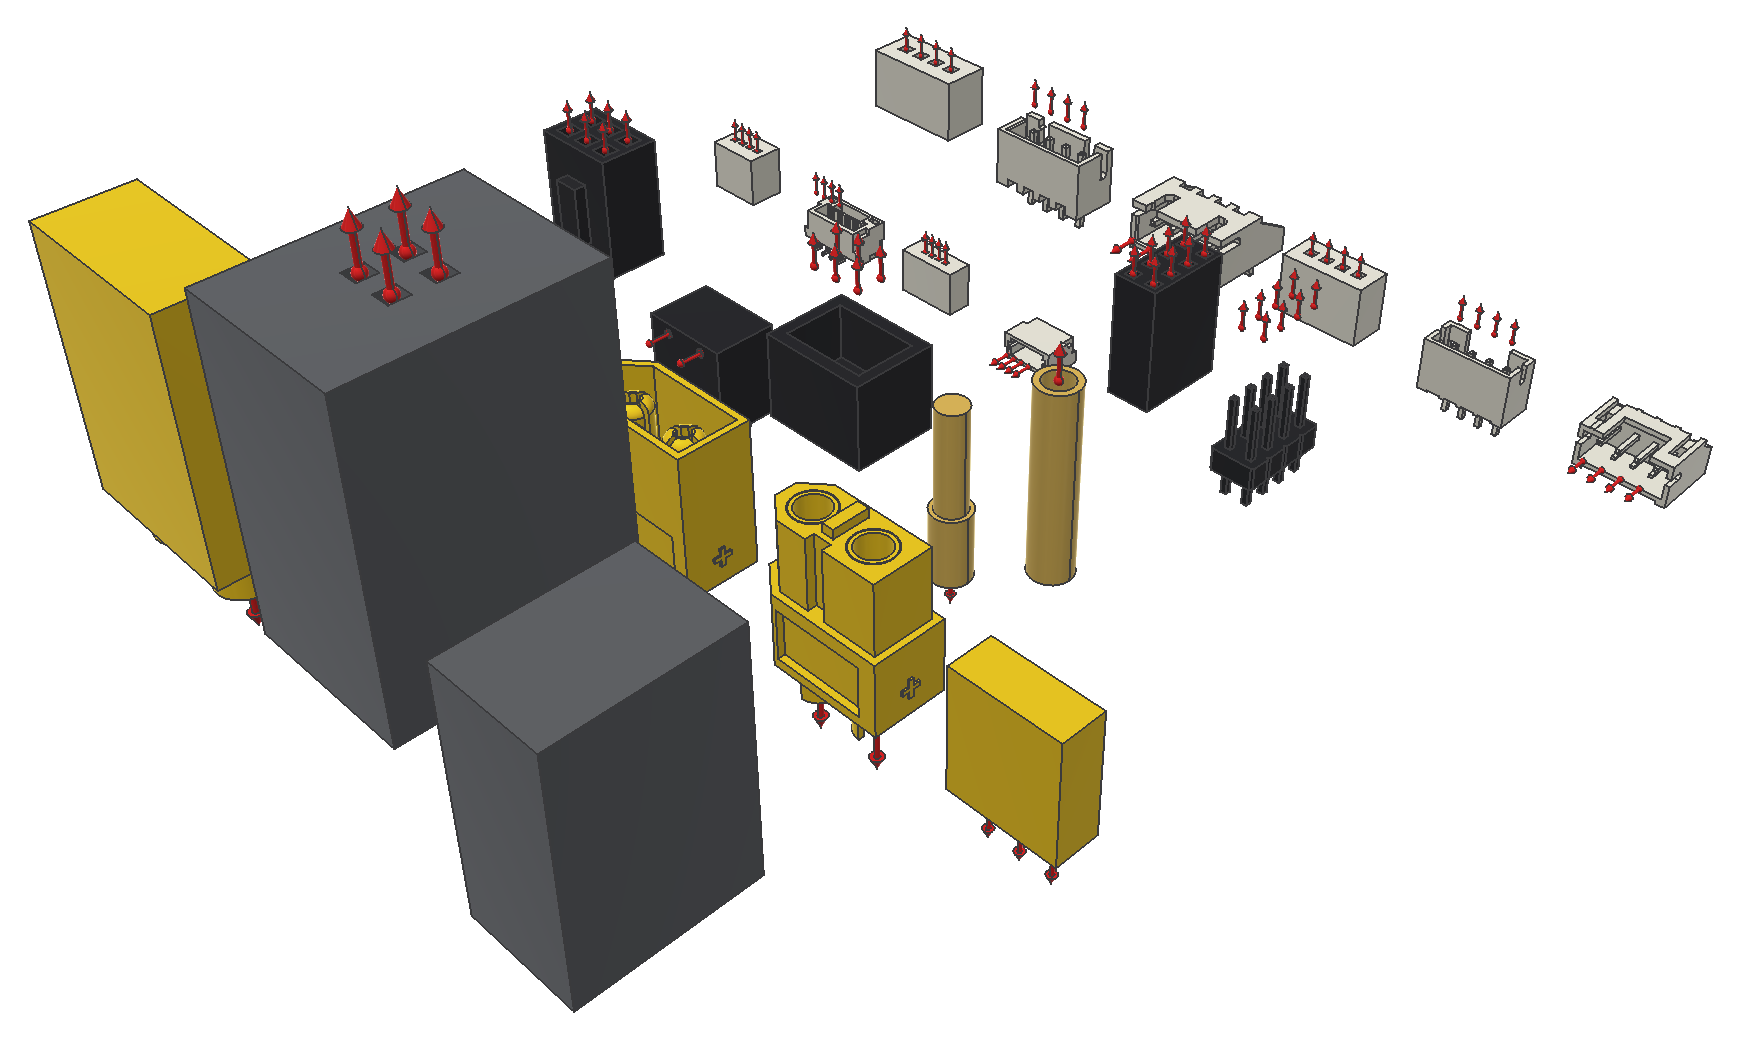
\includegraphics[width=0.92\linewidth]{fig/rou05_connectors.png}
\caption{Generated connector parts, one or two per family, with their pin frames drawn as red arrows along $+Z$ (the
direction the wire leaves). Back rows: JST XH, PH, GH and SH housings with their vertical and right-angle headers
(KiCad models; the housings are parametric), Dupont 2.54\,mm housing and pin header. Middle: Molex Micro-Fit 3.0
receptacle, plug and vertical header, 3.5\,mm bullets. Front: XT30, XT60 (KiCad model), XT90, MR30 and a Deutsch
DT04/DT06 pair; the solder-cup and plug frames point down. Off-screen render of the real part files.}
\label{fig:connlib-built}
\end{figure}

\paragraph{What you have now.}
\begin{itemize}[nosep]
  \item \textbf{159 connector part files}, one \code{App::Part} each, named after the MPN, holding the body and one
        pin frame per contact (figure~\ref{fig:connlib-built}). Each frame's origin is where the wire leaves the
        housing (the rear face of the contact cavity, or the solder-cup mouth), $+Z$ points out along the wire, and
        $+X$ points towards pin~2. The frames carry \code{PinName} (the pad number), \code{GaugeMin}/\code{GaugeMax}
        (AWG), \code{TerminalPN} (the crimp contact, e.g.\ \code{SXH-001T-P0.6} on an XH housing) and \code{SealPN}.
  \item \textbf{Part properties} for the BOM and the vault: the built-in part schema with \code{ItemType}
        \emph{cots}, \code{Description}, \code{Vendor}/\code{VendorPartNumber}; plus \code{Manufacturer},
        \code{ManufacturerPartNumber} (as the KiCad bridge's items have), \code{ConnectorFamily},
        \code{ConnectorRole}, \code{MatingPN} (several mates separated by ``;''), \code{FrameAt}, \code{ConnectorPitch},
        \code{AccessoryPN} (DT wedgelock), \code{Footprint}, and in the \emph{Source} group \code{ModelSource} and
        \code{ModelLicense} (the attribution below).
  \item \textbf{Mating that places itself}: a wire housing uses its vertical header's footprint frame, so a housing
        placed where its header is placed sits mated, and the header's frames lie on the housing's frames
        (\code{FrameAt}~=~\emph{Mated plug}: a wire routed to a header pin ends where it really leaves the mated
        housing). The same holds for the parametric wire-to-wire pairs (Micro-Fit plug/receptacle, DT04/DT06, the
        bullets). A right-angle header's frames are at the mated housing's rear face, pointing along the board.
  \item \textbf{A manifest} (\file{manifest.json} with every value, \file{manifest.csv} one row per part) beside the
        part files, and a vault import: \code{python -m bruceworx.connector\_library import -{}-vault <Standard
        Libraries> -{}-manifest <folder>/manifest.json [-{}-dry-run]} numbers each part as a new \emph{cots} item
        through \code{vault\_setup.new\_item} (as New COTS Item does: number previewed, file made, number taken,
        checked in as WIP~01), writes the P/N and revision into the part under FreeCADCmd, and skips a part whose
        description is already an item, so it can be run again after the library grows.
\end{itemize}

\paragraph{The library.} Pin counts follow your brief: JST 2--8, Micro-Fit 2--12 (dual row), DT 2/3/4/6/8/12, the
power connectors as AMASS makes them.
\begin{center}
\small
\begin{tabularx}{\linewidth}{@{}lrrrX@{}}
\toprule
Family & Parts & KiCad & Param. & Parts and source\\
\midrule
JST XH (2.50) & 21 & 14 & 7 & \code{XHP-n} housing; \code{BnB-XH-A} vertical and \code{SnB-XH-A} right-angle header
  (KiCad); terminal \code{SXH-001T-P0.6}, 28--22\,AWG\\
JST PH (2.00) & 21 & 14 & 7 & \code{PHR-n}; \code{BnB-PH-K}, \code{SnB-PH-K}; \code{SPH-002T-P0.5S}, 30--24\,AWG\\
JST GH (1.25) & 21 & 14 & 7 & \code{GHR-0nV-S}; \code{BM0nB-GHS-TBT}, \code{SM0nB-GHS-TB}; \code{SSHL-002T-P0.2},
  30--26\,AWG\\
JST SH (1.00) & 21 & 14 & 7 & \code{SHR-0nV-S-B}; \code{BM0nB-SRSS-TB}, \code{SM0nB-SRSS-TB}; \code{SSH-003T-P0.2-H},
  32--28\,AWG\\
Dupont 2.54 & 28 & 14 & 14 & Amphenol FCI Mini-PV housings \code{65039-0xxLF} ($1\times2$--$1\times8$),
  \code{65043-0xxLF} ($2\times2$--$2\times8$); male pin headers (KiCad, generic); \code{48235-000LF}, 26--22\,AWG\\
Micro-Fit 3.0 & 18 & 0 & 18 & \code{43025} receptacle, \code{43020} plug, \code{43045-xx12} vertical header (pads from
  KiCad, no model installed); \code{43030-0007}/\code{43031-0007}, 24--20\,AWG\\
XT30 & 4 & 0 & 4 & \code{XT30U-M/F}, \code{XT30PW-M/F} (pads from KiCad); solder cup, 18--16\,AWG\\
XT60 & 4 & 2 & 2 & \code{XT60-M/F} (KiCad models), \code{XT60PW-M/F}; 14--12\,AWG\\
XT90 & 3 & 0 & 3 & \code{XT90H-M/F}, \code{XT90PW-M}; 10--8\,AWG\\
MR30 & 4 & 0 & 4 & \code{MR30-M/F}, \code{MR30PW-M/FB}; 18--16\,AWG\\
Bullet 3.5\,mm & 2 & 0 & 2 & male and female, solder cup, 16--14\,AWG (generic)\\
Deutsch DT & 12 & 0 & 12 & \code{DT04-nP} receptacle (pin \code{0460-202-16141}), \code{DT06-nS} plug (socket
  \code{0462-201-16141}); 20--16\,AWG; wedgelocks \code{WnP}/\code{WnS}; no per-wire seal\\
\midrule
Total & 159 & 72 & 87 & every mating pair symmetric; plus 22 terminals, seals and wedgelocks (below)\\
\bottomrule
\end{tabularx}
\end{center}

\paragraph{Where KiCad has no model (parametric fallback).} The installed KiCad 10 library (3.1\,GB of STEP in the
app bundle; nothing in \file{\textasciitilde/Documents/KiCad}) has only board-side parts. Parametric outlines were
needed for: every \textbf{wire-side housing} (JST XHP/PHR/GHR/SHR, Dupont, Micro-Fit 43025/43020, DT); the
\textbf{Micro-Fit headers}, \textbf{XT30}, \textbf{XT90} and \textbf{MR30} (KiCad has their footprints, so the pins
still come from the pads, but their STEP files are not installed); and the \textbf{bullets} and \textbf{Deutsch DT}
(no footprint either: pins from the family's pitch). The generator picks the KiCad model whenever the STEP file
exists, so installing KiCad's full 3D library and running it again replaces those outlines without other changes.

\paragraph{How the pins are placed.} KiCad's models sit in footprint coordinates with $y$ flipped (all these footprints
have zero model offset and rotation), so pad $(x, y)$ is at $(x, -y, 0)$ in the part; pads without a number or named
\code{MP} (pegs, mounting pads) are not pins. The wire-entry heights and lengths of the JST families are from the JST
datasheets: mated height above the board 9.8\,mm (XH), 8\,mm (PH), 7.3\,mm (GH), 6.3\,mm (SH); right-angle mated
length from the header's rear edge 14.3, 9.6, 7.15 and 6.25\,mm.

\paragraph{Licence.} KiCad's 3D models are CC-BY-SA~4.0 with the KiCad libraries exception: a design that uses them
is not ``Adapted Material'', so your assemblies and boards are free of the licence; the connector part files that
embed a model are adapted copies and carry the attribution. Each KiCad-model part has in \code{ModelLicense}:
\emph{``KiCad library 3D model, CC-BY-SA 4.0 with the KiCad libraries exception (designs using it are not Adapted
Material; https://www.kicad.org/libraries/license/). Attribution: KiCad Library Team and contributors,
kicad-packages3D.''} and in \code{ModelSource} the model's library path. Parametric parts say so in both fields.
Distributing the library parts themselves (not designs) should keep that notice and the CC-BY-SA terms.

\paragraph{Decided while building.}
\begin{itemize}[nosep]
  \item \textbf{One part per MPN}, not one part with a pin-count parameter: each is its own vault item with its own
        P/N and mates by MPN.
  \item \textbf{Headers get frames} at the mated housing's rear face (\code{FrameAt}~=~\emph{Mated plug}, agreed with
        rou05), so routing to a board connector works before the wire-side housing is placed.
  \item \textbf{Dupont} housings are the original, Amphenol FCI Mini-PV (clones fit); the male pin headers stay
        generic (\code{HDR254-M-1x04}); female-crimp housings on male headers only.
  \item \textbf{DT seal}: the DT wire seal is the one-piece rear grommet inside the housing, so the pins have no
        \code{SealPN}; \code{114017}, the sealing plug for an unused cavity, is a library part named in the notes.
  \item \textbf{Colours} are stored: the library is built by the GUI FreeCAD (off screen), and the import puts the
        view data back after FreeCADCmd numbers the copy (\code{restore\_view\_data}).
  \item \textbf{Import} through \code{vault\_setup.new\_item} with kind \emph{cots} (the Standard Libraries' type),
        not \code{vault import}, which numbers files as \emph{part}; the vault files themselves are unchanged.
\end{itemize}

\paragraph{Tests.} FreeCAD-free (\file{addons/BruceWorx/tests/test\_connector\_library.py}, 17 tests, 0.1\,s): the
tables, unique MPNs, files and descriptions, every family present with its pin counts, mating symmetric with equal pin
counts, gauge ranges the right way round, terminals and seals, pins from the pads (GH pegs left out, KiCad $y$ flipped,
Micro-Fit's two rows), wire directions, the KiCad models resolving, the manifest round trip, and the import and dry
run on a scratch vault (numbers, \emph{cots}, the writer called, nothing staged left, a second run importing nothing).
FreeCAD headless (\file{TestBruceWorxConnectorLibrary}, 7 tests): twelve generated parts reopened from disk have
$N$ frames read by rou05's \code{pins()} with the schema's properties, the pad names and positions, $+Z$ pointing away
from the body (frame origin beyond the body's bounding-box centre along $+Z$, a point 1\,mm out along $+Z$ outside the
box, housing frames on the box face), the KiCad body with its licence note and the XH header's 7.0\,mm height, the
housing mating its header at the same placement, and the vault scan seeing a part. \textbf{Import dry run}: on a copy
of your Standard Libraries vault (the real one only read) the dry run numbers the 159 parts
\code{STD-01-01004-001} to \code{STD-01-01162-001}; the real import into the copy then checked all 159 in as
\emph{cots} items with the P/N and revision written into each file (1.8\,s), and a second dry run finds nothing left to
import.

\paragraph{Not done.} Importing into the real Standard Libraries vault (waits on you); fittings (F1, a separate
piece); terminals and seals as their own vault items (the pins name them by manufacturer P/N for now); Dupont
male-crimp housings and pin sockets; JST 1-pin and $>8$-pin, single-row Micro-Fit (43645/43650).

\paragraph{Open questions for you.}
\begin{center}
\small
\begin{tabularx}{\linewidth}{@{}lXX@{}}
\toprule
\# & Question & Built for now (recommendation)\\
\midrule
1 & Import the 159 parts into the real Standard Libraries now (\code{STD-01-01004-001} \dots{} \code{-01162-001})?
  & Waiting on you; the command is above.\\
2 & Install KiCad's full 3D library (or download Micro-Fit, XT30/XT90/MR30 STEP files) to replace 87 parametric
  outlines? & Parametric; regenerate once the models are there.\\
3 & Terminals and seals as vault items with their own P/N (so the C3 terminal BOM lines carry a P/N), or manufacturer
  P/N on the pin? & Manufacturer P/N on the pin; vault items when the harness BOM (ROU-06) needs them.\\
4 & The approximate dimensions (Micro-Fit, Dupont, XT, MR30, DT; DT pin numbering and 3-way in-line layout): check
  against the datasheets before the harness drawings rely on them? & Approximate, about $\pm1$\,mm.\\
5 & JST crimp: \code{SXH-001T-P0.6} (28--22\,AWG) as the XH default, or \code{SXH-002T-P0.6} (30--26) for thin wire?
  & 001T; the other is in the notes.\\
\bottomrule
\end{tabularx}
\end{center}

%----------------------------------------------------------------------
\subsubsection*{Answers and follow-up (30 Oct)}

\begin{center}
\small
\begin{tabularx}{\linewidth}{@{}lXX@{}}
\toprule
\# & Your answer & What was done\\
\midrule
1 & Import into the real Standard Libraries: approved; the vault stays on the Extreme SSD; the main session runs it
  with Keystone closed, after a backup. & Not run here (single writer). Library, manifest and the command below;
  a fresh dry run on a fresh copy numbers all 181 parts.\\
2 & Install KiCad's 3D models to replace the outlines. & Nothing to install: see below. Still 87 outlines.\\
3 & Terminals and seals by manufacturer P/N; STD numbers for finding. & 22 terminals, seals and wedgelocks are
  library parts; pins carry MPN and manufacturer, and the STD number after import; the ordering list prints
  manufacturer and MPN.\\
4 & Check Micro-Fit, Dupont, XT, MR30 and DT against the datasheets. & Done where the drawings could be had;
  tables fixed (below), estimates marked.\\
5 & Keep \code{SXH-001T-P0.6} as the XH crimp. & Kept.\\
-- & Save view colours if cheap. & Done: GUI build, colours kept through the import.\\
\bottomrule
\end{tabularx}
\end{center}

\paragraph{KiCad models (answer 2).} The connector folders of the official library
(\file{kicad-packages3D} on GitLab) were compared with what is installed: the tags \code{10.0.8} (KiCad~10's library;
the app is 10.0.5), \code{9.0.3} back to \code{5.1.12}, and the \code{dev} branch. The installed
\file{Connector\_JST}, \file{Connector\_Molex}, \file{Connector\_AMASS} and the 2.54\,mm pin header and socket folders
are \emph{identical} to 10.0.8 (158, 89, 2, 278, 278 STEP files), and no tag or branch has a model for a Micro-Fit
part, XT30, XT90, MR30, any JST wire housing or Deutsch DT (\file{Connector\_AMASS} has only the two XT60 models; TE has
no DT). So nothing was downloaded and KiCad's setup is untouched; the 87 parametric connector outlines stay (28 JST housings, 14 Mini-PV
housings, 18 Micro-Fit, 13 XT30/XT60PW/XT90/MR30, 2 bullets, 12 DT), and the 22 terminals, seals and wedgelocks
are simple outlines too. Real bodies for them would have to come
from the manufacturers' STEP files (Molex, TE, AMASS; behind logins and their own licences) --- question~6.

\paragraph{Terminals, seals, wedgelocks (answer 3).} Agreed with rou05 as schema v1.2:
\begin{itemize}[nosep]
  \item each crimp pin has \code{TerminalPN} (the manufacturer's P/N, for ordering), \code{TerminalMfr} and
        \code{TerminalItem} (its Standard Library P/N, for finding); \code{SealPN}/\code{SealMfr}/\code{SealItem} the
        same; a DT connector lists its wedgelock in \code{Accessories} (\code{MPN|manufacturer|STD item|qty|kind});
  \item the 22 parts are \emph{cots} items of their own with \code{Manufacturer}, \code{ManufacturerPartNumber} and
        \code{AccessoryKind}: the JST, Mini-PV and Micro-Fit crimp terminals, the two Deutsch size-16 contacts, the
        \code{114017} sealing plug and the twelve wedgelocks \code{W2P}\ldots\code{W12S};
  \item the import numbers them first, then writes their STD numbers into every connector's pins and
        \code{Accessories} as it checks the connector in; a terminal already in the vault keeps its number;
  \item the import writes \file{vault\_numbers.csv} beside the manifest (vault P/N, manufacturer, MPN, description,
        role): the list to order from. rou05's BOM keys the terminal lines by the STD item and prints
        manufacturer and MPN.
\end{itemize}

\paragraph{Dimensions checked (answer 4).} Sources: Molex \emph{SD-43025-002} (receptacle) and the product pages of
\code{43045-0212}/\code{-1415}; FCI customer drawing \emph{65043} rev.\,BG (Mini-PV dual row); the AMASS XT catalogue
(Feb~2026, china-amass.com) and AMASS spec sheets for \code{XT30PW-M}, \code{XT60PW-M}, \code{XT90PW-M},
\code{MR30PW-M}; the Deutsch industrial catalogue and TE drawing \emph{C-2286003} (\code{DT06-2S}). Molex, TE and
Amphenol block scripted downloads, so the PDFs were read from distributor mirrors of the manufacturers' own
drawings (chipdip, comet.bg, LCSC, onlinecomponents). What changed:
\begin{center}
\small
\begin{tabularx}{\linewidth}{@{}lXX@{}}
\toprule
Family & Was & Now (source)\\
\midrule
Micro-Fit & receptacle $3c{+}3.6$ wide, 9.85 deep, 10.6 long; wire face 12.6 above the PCB & $3c{+}0.85$ wide
  ($c$ columns), 6.86 deep (7.57 for 2 and 4 circuits), 14.0 long, latch on the row-2 side; wire face
  \textbf{17.64} above the PCB (Molex mated height); plug 10.77 beyond the mating face (24.77 mated)\\
Dupont & generic housings \code{DUPONT-HSG-\ldots}, generic terminal, 14.0 tall & Amphenol FCI Mini-PV
  \code{65039-0xxLF} / \code{65043-0xxLF}, 13.84 tall, 5.08 deep (dual); contact \code{48235-000LF}, 26--22\,AWG;
  wire face 16.38 above the PCB\\
XT30 / XT60 & one length per family & per MPN: \code{XT30U-M} 13.7, \code{-F} 12.4, cups 3.0; XT60 20.5/20.2\\
XT90 & \code{XT90-M/F}, pitch 10.9 & \code{XT90H-M/F} (the current AMASS parts), pitch 11.0, 30.7/29.7 long\\
MR30 & 13.0 wide, cups 4.0 & 11.9 wide, 4.9 thick, bodies 13.4/12.4, cups 2.0\\
PCB (PW) & body length from the KiCad pegs & AMASS heights and pin-to-face lengths (\code{XT30PW-M} 5.2 / 13.05,
  \code{XT60PW-M} 8.4 / 14.7, \code{XT90PW-M} 10.2 / 24.6, \code{MR30PW-M} 4.9 / 13.05)\\
Deutsch DT & pitch 5.0 everywhere, 3-way in line, seal \code{114017} on every pin & spacing 5.46 (2-way), 4.45--4.47
  (others), \textbf{3-way triangular}, plug \code{DT06-2S} $15.0\times15.8\times28.8$; \textbf{no per-wire seal}
  (one-piece rear grommet); contacts 20--16\,AWG\\
\bottomrule
\end{tabularx}
\end{center}
Still estimates (marked in the generator): the 43045 vertical header's own body and the 43020 plug's width; the
single-row Mini-PV suffixes \code{-034LF} and \code{-029LF} (inferred from the dual-row pattern) and its depth; the
mated cup position of the XT30/XT90/MR30 PCB parts and the female PW lengths; the DT receptacle outline, the 3-way
triangle size and the DT cavity numbering (1\ldots$k$ along one row and back along the other); 43031-0007's AWG range.

\paragraph{The library now.} 181 parts: 159 connectors (unchanged list but \code{XT90H}, the Mini-PV MPNs) and 22
terminals, seals and wedgelocks; built by the GUI FreeCAD off screen in 18\,s, 4.8\,MB, every file with its colours.
Commit \code{323ec9bb}.

\paragraph{Import command (for the main session; Keystone closed, vault backed up).} The library is in the connlib
scratch folder (\file{agent-connlib/library/}). From the repository:
\begin{center}
\small
\code{BW\_CONNLIB\_ARGS="import -{}-vault '<Standard Libraries>' -{}-manifest <library>/manifest.json"}\\
\code{build/release/bin/FreeCADCmd -u <cfg> <script that calls bruceworx.connector\_library.main()>}
\end{center}
(FreeCADCmd so the P/N, the revision and the STD numbers are written into each file; \code{-{}-dry-run} first). A fresh
dry run on a fresh copy of your vault (3 items, next parent 1004) numbers the terminals, seals and wedgelocks
\code{STD-01-01004-001} \ldots{} \code{STD-01-01025-001} and the connectors \code{STD-01-01026-001} \ldots{}
\code{STD-01-01184-001}. The full import into that copy took 3\,s: 184 items, \code{XHP-4} with
\code{TerminalItem}~=~\code{STD-01-01004-001}, \code{DT04-4P} with its wedgelock \code{W4P} as
\code{STD-01-01018-001}, colours kept; a second dry run finds nothing left to import.

\paragraph{Tests.} FreeCAD-free 20 (new: accessories as parts with their manufacturers, every pin's terminal a
library part, accessories numbered first and their numbers handed to the pins, the ordering list, the view data
restored, the DT layouts and the checked values); headless FreeCAD 9 (new: terminal and wedgelock parts, the pins'
\code{TerminalMfr}, \code{Accessories}, \code{fill\_items} on a DT connector). All pass.

\paragraph{New open questions.}
\begin{center}
\small
\begin{tabularx}{\linewidth}{@{}lXX@{}}
\toprule
\# & Question & Built for now (recommendation)\\
\midrule
6 & The 87 outlines: download the manufacturers' STEP files (Molex 43025/43020/43045, AMASS XT30/XT90/MR30, TE
  DT) by hand, under their licences, and let the generator use them? & Outlines; the frames would need checking
  against each model's origin, so one family at a time.\\
7 & Pin headers: pick a real MPN (e.g.\ a Samtec or Amphenol 2.54\,mm header) so the board side orders by MPN too?
  & Generic for now.\\
8 & DT cavity numbering: confirm against a TE customer drawing (te.com blocks scripted downloads). & Estimated.\\
\bottomrule
\end{tabularx}
\end{center}
